\subsection{Algorithmen}
\label{sec:Algorithmen}

\begin{itemize}
	\item Abbildung der Kontrollstrukturen mittels Struktogramm, PAP oder Pseudocode als didaktisches Hilfsmittel
	\item grundlegende Algorithmen kennen, eigene Algorithmen auch programmiersprachenfrei formulieren und zur Lösung von Problemen, z.B. in einem IT-System bzw. einer Softwareanwendung einsetzen
	\item Entwickeln und Darstellen von Programmlogiken unabhängig von der Programmiersprache, z.B. mithilfe von Struktogrammen nach Nassi-Shneidermann sowie Strukturdiagrammen und Verhaltensdiagrammen aus der UML
	\item Rekursion: Funktionsweise, Vor-/Nachteile
	\item Algorithmen implementieren/durchspielen
	\begin{itemize}
		\item Mittelwert
		\item doppelte Einträge in einem Array finden/löschen
		\item Dateibäume rekursiv kopieren
		\item (Zinses-)Zinsberechnung
		\item Planen eines regelmäßigen Backups
		\item Ablauf einer Benutzerauthentifizierung an einer Website
		\item Abbuchen von einem Konto
		\item Lineare Suche
		\item Binäre Suche
		\item Bubble Sort
	\end{itemize}
\end{itemize}

\subsubsection{Flussdiagramm}
\label{sec:Flussdiagramm}

\begin{multicols}{2}
	\begin{center}
		\begin{tikzpicture}[node distance=1cm]
			\node (start) [startstop] {Start/Ende};
			\node (process) [process, below=of start] {Prozess-/Tätigkeitssymbol};
		\end{tikzpicture}
	\end{center}
	
	\begin{center}
		\begin{tikzpicture}[node distance=1cm]
			\node (io) [io] {Eingabe/Ausgabe};
			\node (decision) [decision, below=0.3cm of process, shape aspect=2] {Entscheidungssymbol};
			\draw [arrow] (io) -- node[anchor=east] {Verbindungspfeil} (decision);
		\end{tikzpicture}
	\end{center}
\end{multicols}

\newpage

\subsubsection{Struktogramm (Nassi-Shneiderman-Diagramm)}
\label{sec:Struktogramm}

Quelle: Lehrerfortbildung-bw.de \cite{Struktogramm}

\begin{minipage}[c]{0.25\textwidth}
	Anweisung
\end{minipage}
\begin{minipage}[c]{0.65\textwidth}
	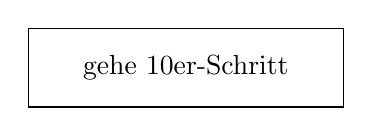
\begin{tikzpicture}[node distance=0cm]
		\node[minimum height=1cm, minimum width=4cm, draw]{gehe 10er-Schritt};
	\end{tikzpicture}
\end{minipage}

\hfill

\begin{minipage}[c]{0.25\textwidth}
	Sequenz
\end{minipage}
\begin{minipage}[c]{0.65\textwidth}
	\begin{tikzpicture}[node distance=0cm]
		\node[minimum height=1cm, minimum width=4cm, draw](10erSchritt){gehe 10er-Schritt};
		\node[minimum height=1cm, minimum width=4cm, draw, below=of 10erSchritt](stift){schalte Stift ein};
		\node[minimum height=1cm, minimum width=4cm, draw, below=of stift](sageHi){sage 'Hallo!'};
	\end{tikzpicture}
\end{minipage}

\hfill

\begin{minipage}[c]{0.25\textwidth}
	Schleife mit Bedingung
\end{minipage}
\begin{minipage}[c]{0.65\textwidth}
	\begin{tikzpicture}[node distance=0cm]
		\node[minimum height=2cm, minimum width=5cm, draw](wiederhole){};
		\node[minimum height=2cm, minimum width=5cm, above=-1.5cm of wiederhole](wiederholeText){wiederhole bis Rand berührt};
		\node[minimum height=1cm, minimum width=4cm, draw, below right=-1cm and -4cm of wiederhole](aendere){ändere x um 10};
	\end{tikzpicture}
\end{minipage}

\hfill

\begin{minipage}[c]{0.25\textwidth}
	Schleife mit Zähler
\end{minipage}
\begin{minipage}[c]{0.65\textwidth}
	\begin{tikzpicture}[node distance=0cm, align=center]
		\node[minimum height=3cm, minimum width=5cm, draw](wiederhole){};
		\node[minimum height=2cm, minimum width=5cm, above=-1.5cm of wiederhole](wiederholeText){wiederhole 10 mal};
		\node[minimum height=1cm, minimum width=4cm, draw, below right=-2.1cm and -4cm of wiederhole](gehe){gehe 4er-Schritt};
		\node[minimum height=1cm, minimum width=4cm, draw, below right=-1.1cm and -4cm of wiederhole](drehe){drehe dich nach rechts\\um 5 Grad};
	\end{tikzpicture}
\end{minipage}

\hfill

\begin{minipage}[c]{0.25\textwidth}
	Endlosschleife
\end{minipage}
\begin{minipage}[c]{0.65\textwidth}
	\begin{tikzpicture}[node distance=0cm, align=center]
		\node[minimum height=3cm, minimum width=5cm, draw](wiederhole){};
		\node[minimum height=2cm, minimum width=5cm, above=-1.5cm of wiederhole](wiederholeText){wiederhole fortlaufend};
		\node[minimum height=1cm, minimum width=4cm, draw, below right=-2cm and -4cm of wiederhole](gehe){gehe 8er-Schritt};
		\node[minimum height=1cm, minimum width=4cm, draw, below right=-1cm and -4cm of wiederhole](drehe){pralle vom Rand ab};
	\end{tikzpicture}
\end{minipage}

\hfill

\begin{minipage}[c]{0.25\textwidth}
	Verzweigung mit \\Alternative
\end{minipage}
\begin{minipage}[c]{0.65\textwidth}
	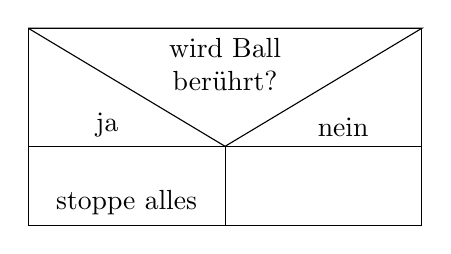
\begin{tikzpicture}[node distance=0cm, align=center]
		\draw (0,0) -- (5,0) node[below,pos=0.5]{wird Ball\\berührt?} -- (2.5,-1.5) -- (0,0);
		\draw (0,0) -- (0,-1.5) -- (2.5,-1.5)node[above,pos=0.4]{ja};
		\draw (0,-1.5) -- (0,-2.5) -- (2.5,-2.5) node[above, pos=0.5]{stoppe alles} -- (2.5,-1.5);
		\draw (5,0) -- (5,-1.5) -- (2.5,-1.5)node[above,pos=0.4]{nein};
		\draw (5,-1.5) -- (5,-2.5) -- (2.5,-2.5) -- (2.5,-1.5);
		
	\end{tikzpicture}
\end{minipage}

\hfill